\chapter{Desenvolvimento}

No capítulo anterior foram mostradas as características, os pontos fortes de cada tecnologia, e também os motivos para sua escolha. Nesse capítulo será descrito a especificação do projeto para o sistema proposto, seu funcionamento e estrutura.

O projeto consiste basicamente, na implementação de uma solução que possibilite a criação de cursos em vídeos com elementos de questões interativas integrado com um sistema de gestão de aprendizado [\autoref{sec:lms}] por meio do \textit{LTI} [\autoref{sec:lti}]. 

O funcionamento do sistema é baseado no modelo cliente/servidor, permitindo que o cliente realize solicitações ao servidor, que então envia os resultados de volta ao cliente, como pode ser vista na figura~\ref{fig:comunicacao-cliente-servidor}.

\begin{figure}[h]
    \centering
    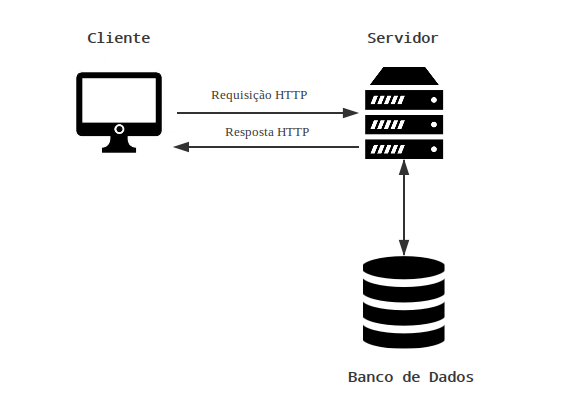
\includegraphics[keepaspectratio=true,scale=0.7]{figuras/comunicacao_cliente_servidor.png}
    \caption{Ilustração da comunicação cliente/servidor}
    \label{fig:comunicacao-cliente-servidor}
\end{figure}

O desenvolvimento foi dividido em três camadas que são: Camada do Servidor, Camada do Banco de Dados e camada de Apresentação, que serão descritas a seguir.

\section{Camada do Banco de Dados}

O banco de dados utilizado foi o \textit{Mysql} (\autoref{sec:mysql}). A modelo conceitual de dados está representado na seguinte DER (Diagrama Entidade-Relacionamento) figura~\ref{fig:diagrama-er}, que é um diagrama que define as entidades de um sistema, e como elas estão relacionadas.

\begin{figure}[h]
    \centering
    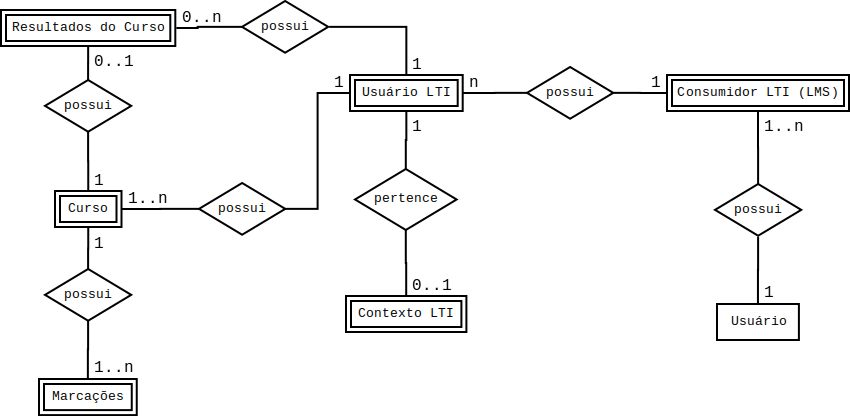
\includegraphics[keepaspectratio=true,scale=0.4]{figuras/der_video_interativo.png}
    \caption{Diagrama ER (Entidade-Relacionamento) do banco de dados.}
    \label{fig:diagrama-er}
\end{figure}

\subsection{Estrutura do banco de dados}

A partir da elaboração do DER, mostrando uma visão geral do relacionamento entre os dados, é possível definir a estrutura do banco de dados, criando uma tabela para cada entidade, e definindo os atributos necessários, formando assim um modelo físico, representando na figura~\ref{diagrama-fisico}.

\begin{figure}[h]
    \centering
    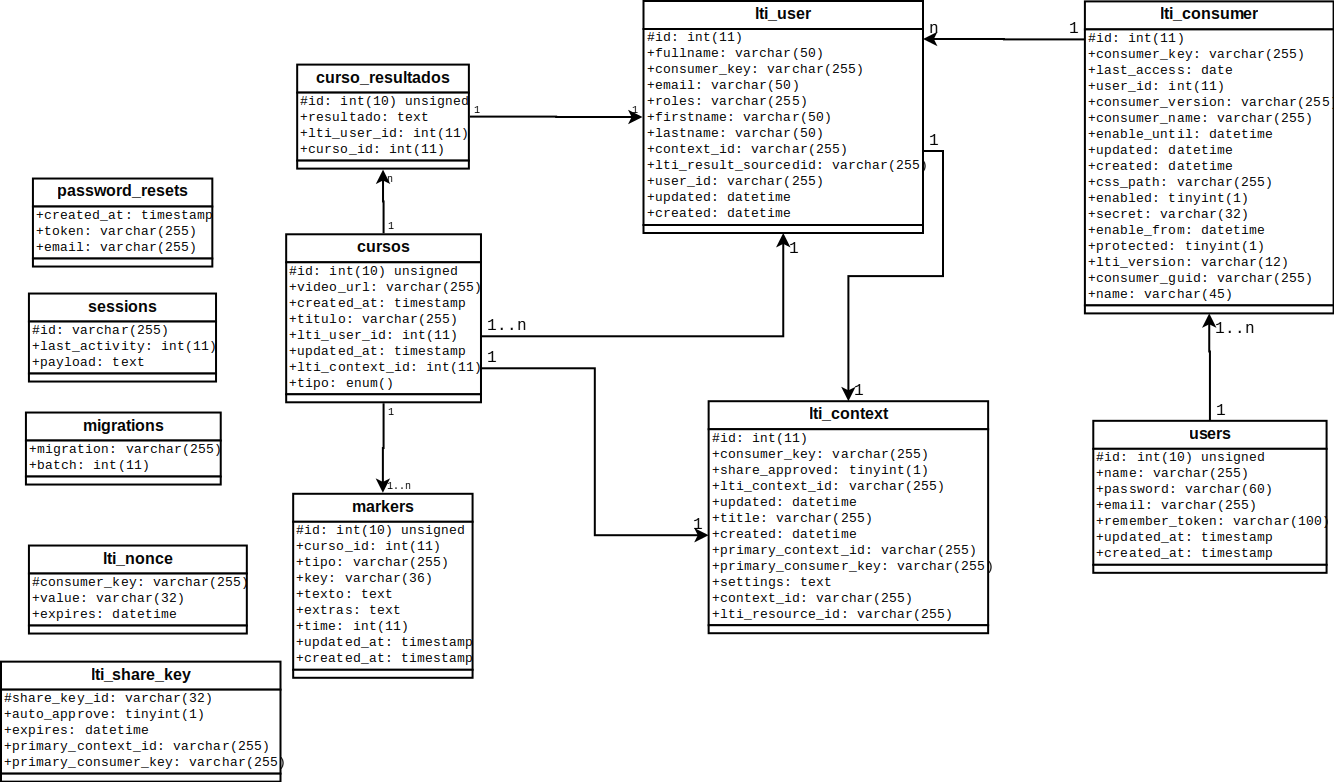
\includegraphics[keepaspectratio=true,scale=0.35]{figuras/modelo_fisico_video_interativo.png}
    \caption{Representação do modelo físico do banco de dados.}
    \label{fig:diagrama-fisico}
\end{figure}

Dessa forma foi definida a estrutura do banco de dados que serão apresentadas nas tabelas TODO. Para cada tabela é mostrado uma breve descrição da sua função, e de seus atributos relevantes para entender a integração explicada em TODO.
\begin{table}[htp]
    \begin{center}
        \begin{tabular}{|c|p{11cm}|}
            \hline \textbf{Tabela} & \textbf{Descrição} \\
            \hline \textit{users} &
                Essa tabela guarda os dados do usuário criado pelo sistema de registro, os usuários dessa tabela são donos de um ou mais \textit{Tool Consumer}, definidos na tabela \textit{lti\_consumer}.
             \\ 
            \hline \textit{lti\_consumer} &
                Armazena os dados do \textit{Tool Consumer} ou seja do sistema \textit{LMS}, como o nome, chave e segredo.
                
                Atributos Importantes:
                \begin{itemize}
                    \item \textit{consumer\_key}: chave do \textit{tool consumer}, gerada pelo sistema, necessária para realizar a autenticação lti.
                    \item \textit{secret}: chave secreta gerada pelo sistema, também necessária para realizar a autenticação \textit{lti}.
                    \item \textit{user\_id}: ligação da tabela com o usuário.
                    \item \textit{consumer\_guid, consumer\_name, consumer\_version, lti\_version}: dados enviados pelo \textit{tool consumer}, por meio da integração \textit{lti}. Correspondem respectivamente à: identificador único do \textit{consumer}, nome, versão e versão do \textit{lti} usada pelo \textit{TC}.
                \end{itemize}
              \\ 
              \hline \textit{lti\_user} &
                  Armazena as informações do usuário do \textit{LMS} (\textit{Tool Consumer}), como seu nome, email e papel.
                  
                  Atributos Importantes:
                  \begin{itemize}
                      \item \textit{consumer\_key}: ligação com tabela \textit{lti\_consumer}.
                      \item \textit{context\_id}: ligação com a tabela \textit{lti\_context}.
                      \item \textit{user\_id firstname, lastname, fullname, email}: dados de perfil enviados pelo \textit{LMS}.
                      \item \textit{roles}: papel do usuário no contexto do \textit{LTI}, exemplo, se ele é professor ou aluno do curso.
                      \item \textit{lti\_result\_sourcedid}: dados gerais da integração necessária para a \textit{API} do \textit{LTI}.
                    \end{itemize}
              \\
              \hline \textit{lti\_context} &
                  Guarda as informações da integração do \textit{LTI}, e da ligação com os cursos.
                  
                  Atributos Importantes:
                  \item \textit{lti\_context\_id}: o id do contexto é equivalente ao id do curso no \textit{LMS}.
                  \item \textit{context\_id e lti\_resource\_id}: guardam a informação do recurso, ou seja a instância única do curso que é ligada ao curso do \textit{Tool Provider}.
                  \\
            \hline 
    \end{tabular} 
    \caption{Tabela com a descrição da tabelas do banco de dados.}
    \label{tbl:estrutura-banco-dados}
    \end{center}
\end{table}

\section{Camada do Servidor}

Esta camada foi desenvolvida utilizando o o servidor \textit{Apache}, descrito na \autoref{sec:apache}, na linguagem \textit{PHP} (\autoref{sec:php}), e para facilitar e estruturar o desenvolvimento, foi usado o \textit{framework Laravel}, que como descrito na \autoref{sec:laravel}, e baseado no padrão arquitetural \textit{MVC} (\autoref{sec:mvc}) que tem como objetivo criar uma independência e a divisão de responsabilidades das partes que envolvem o sistema.

Na camada do servidor, as partes mais importantes do \textit{MVC} são os \textit{Controllers}, que recebem as requisições do cliente e os \textit{Models} que realizam a comunicação com a camada de Banco de Dados.

Os \textit{Controllers} do projeto foram separados da seguinte forma:

\begin{tabular}{|c|p{10cm}|}
    \hline \textbf{Controller} & \textbf{Descrição} \\ 
    \hline \textit{AuthController} & 
        Esse \textit{controller} tem o papel de gerenciar as autenticações simples do sistema, criar e validar as contas. O \textit{controller} foi gerado pelo \textit{Laravel} que contém um modulo de autenticação, mais foi necessário modifica-lo para adicionar a criação da chave do consumidor da integração do \textit{LTI}, ou seja, quando um usuário novo cria uma conta, o sistema precisa gerar também uma chave que será usada para se conectar ao \textit{LMS}.
     \\ 
    \hline \textit{HomeController} & 
        Tem a simples função de criar uma rota para a página inicial do sistema.
     \\ 
    \hline \textit{CursosController} & 
        Tem responsabilidade de tratar as requisições \textit{REST} enviadas pelo cliente para o cadastro e realização do curso.
     \\ 
    \hline \textit{LtiController} & 
        As requisições \textit{LTI} feitas pelo \textit{LMS} passam primeiro por esse \textit{controller}, na ação \textit{launch} (lançamento) onde é feita a comunicação com a \textit{API} do \textit{LTI}.
     \\ 
    \hline 
\end{tabular} 

Os modelos (\textit{models}), são os objetos que proporcionam a comunicação com o banco de dados, tais como consultas e persistência dos dados. O acesso ao banco de dados é feita utilizando a \textit{ORM Eloquent} que como mostrado na \autoref{sec:laravel} consiste em uma \textit{API} de abstração na comunicação com o banco, proporcionando também a abstração dos \textit{drivers} utilizados, ou seja, o mesmo código funcionará para qualquer banco de dados suportado pelo \textit{framework}.

